\chapter{Performance Optimizations}\label{gen:sec:optimizations}
\markboth{Performance Optimizations}{Performance Optimizations}

\newcommand{\nonblockedMethodFigure}{
\begin{figure}[h]
    \centering
    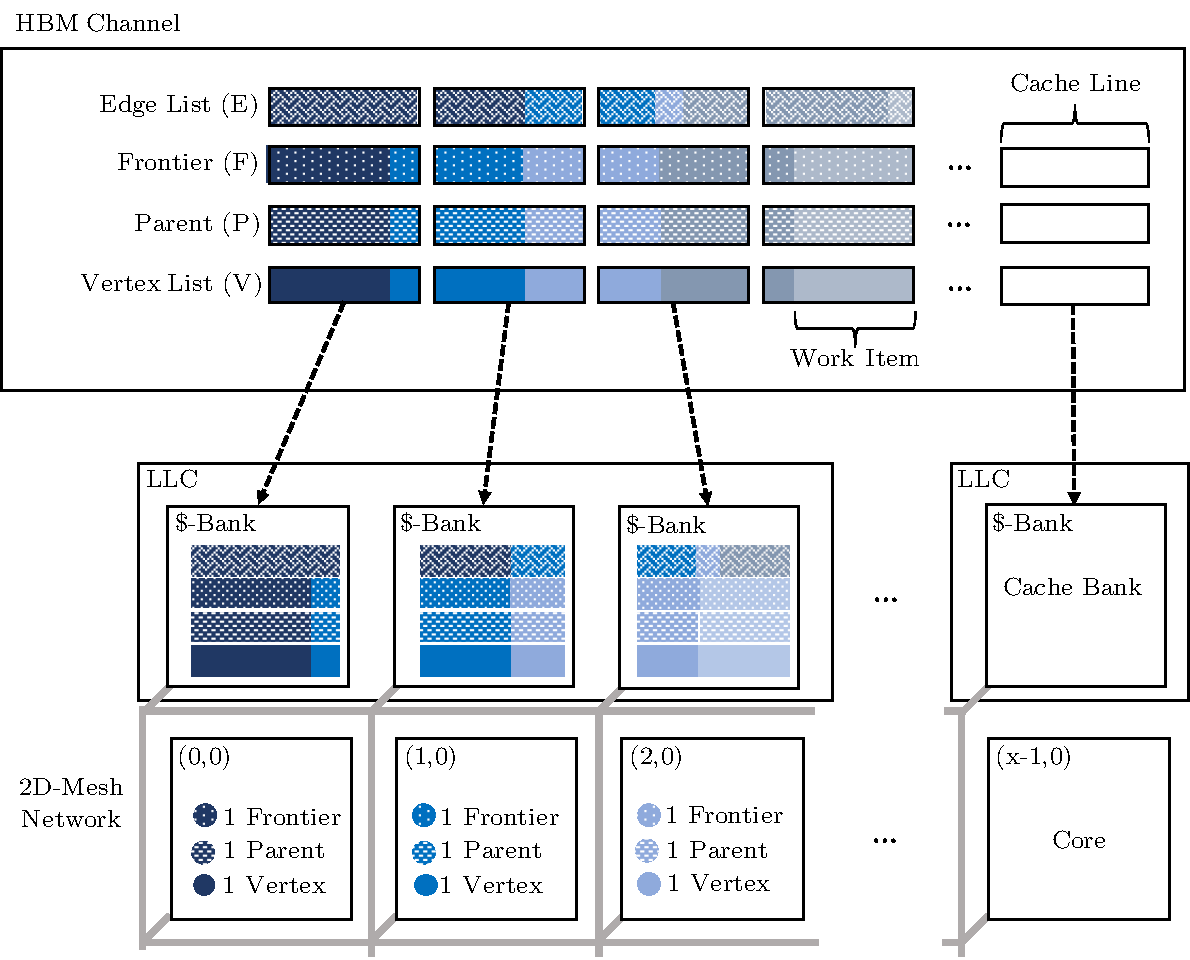
\includegraphics[scale=0.7]{graphit-figures/non-blocked.pdf}
    \caption{Data layout of BFS on the manycore. Data resides in HBM main memory and is cached in LLC. Each core is assigned work items sized without alignment consideration. Cores request single words of data on demand when needed. }
    \label{pap:generals:sec:method:sub:blocked:fig:non-blocked}
\end{figure}
}

\newcommand{\blockedMethodFigure}{
\begin{figure}[t]
    \centering
    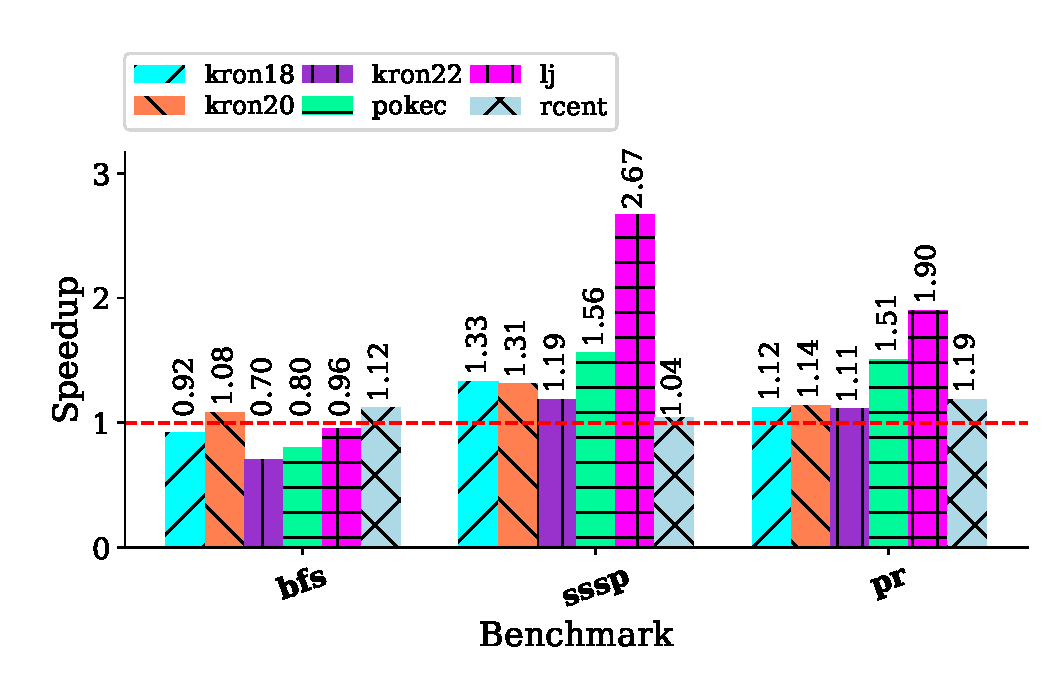
\includegraphics[scale=0.7]{graphit-figures/blocked.pdf}
    \caption{Data layout of BFS with blocked accesses. Cores are assigned cache aligned work items. Cores prefetch entire cache line-sized blocks of data to hide request latency.}
    \label{pap:generals:sec:method:sub:blocked:fig:blocked}
\end{figure}
}

\newcommand{\combinedBlockingFigure}{
\begin{figure*}[t!]
    \centering
    \subfloat[Non-Blocked Accesses]{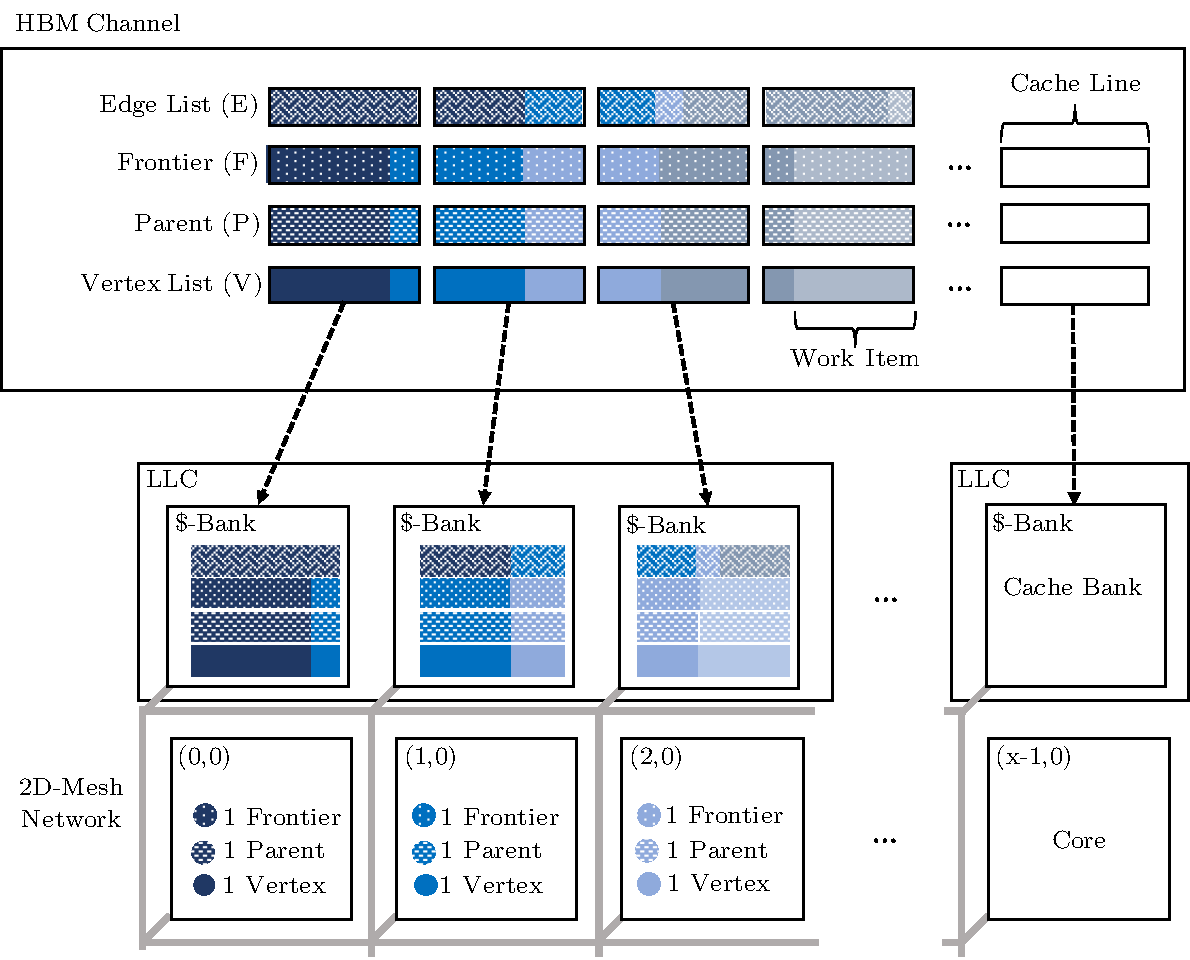
\includegraphics[scale=0.7]{graphit-figures/non-blocked.pdf}}
    \qquad
    \subfloat[Blocked Accesses]{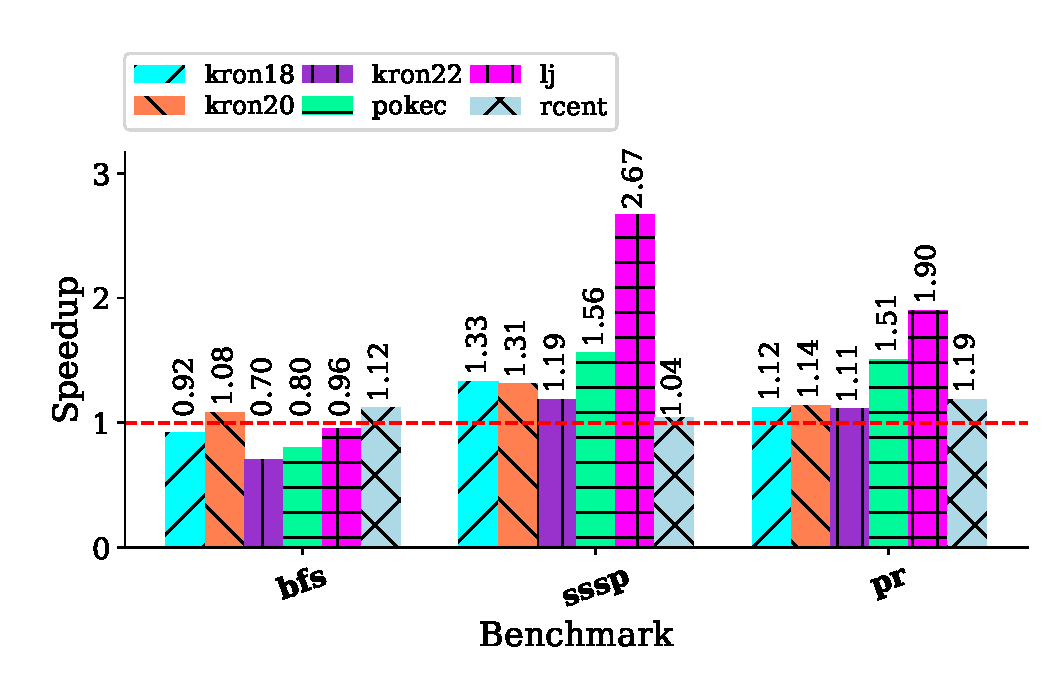
\includegraphics[scale=0.7]{graphit-figures/blocked.pdf}}
    \caption{Data layout of BFS on the manycore. Data resides in HBM main memory and is cached in LLC. In the baseline implementation, each cores are assigned work items sized without alignment consideration and request single words of data on demand when needed. With the blocked access optimization, cores are assigned cache aligned work items and prefetch entire line-sized blocks of data to hide request latency.}
    \label{pap:generals:sec:method:sub:blocked:fig:blocking}
\end{figure*}
}

\newcommand{\edgeAwareMethodFigure}{
\begin{figure}
    \centering
    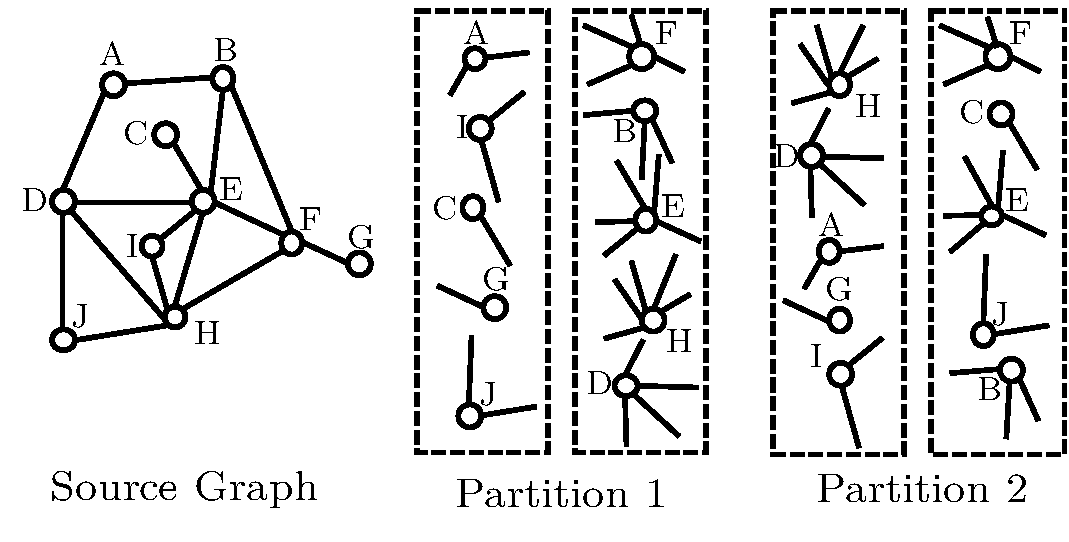
\includegraphics[scale=0.6]{graphit-figures/edge-aware.pdf}
    \caption{Depiction of vertex-based and edge-aware vertex-based partitioning. Partition 1 shows an example vertex-based partitioning between two cores, and Partition 2 shows an example edge-aware partitioning that provides a better workload balance between the two cores.}
    \label{fig:edgeaware}
\end{figure}
}
\newcommand{\edgeAwareMethodAlgorithm}{
\begin{figure}
\centering
\begin{algorithmic}[1]
\Function{Recursive Range}{$start, end$}
\If {$index[end] - index[start] < grain size$}
    \State $core.start \gets start$
    \State $core.end \gets end$
\Else 
    \State $recursive range (start, end/2)$
    \State $recursive range (end/2, start)$
\EndIf
\EndFunction
\end{algorithmic}
\caption{Pseudocode for the recursive call portion of the edge-aware vertex partitioning scheme.}
    \label{alg:edge-aware}
\end{figure}
}
\newcommand{\pushVPullMethodFigure}{
\begin{figure}
    \centering
    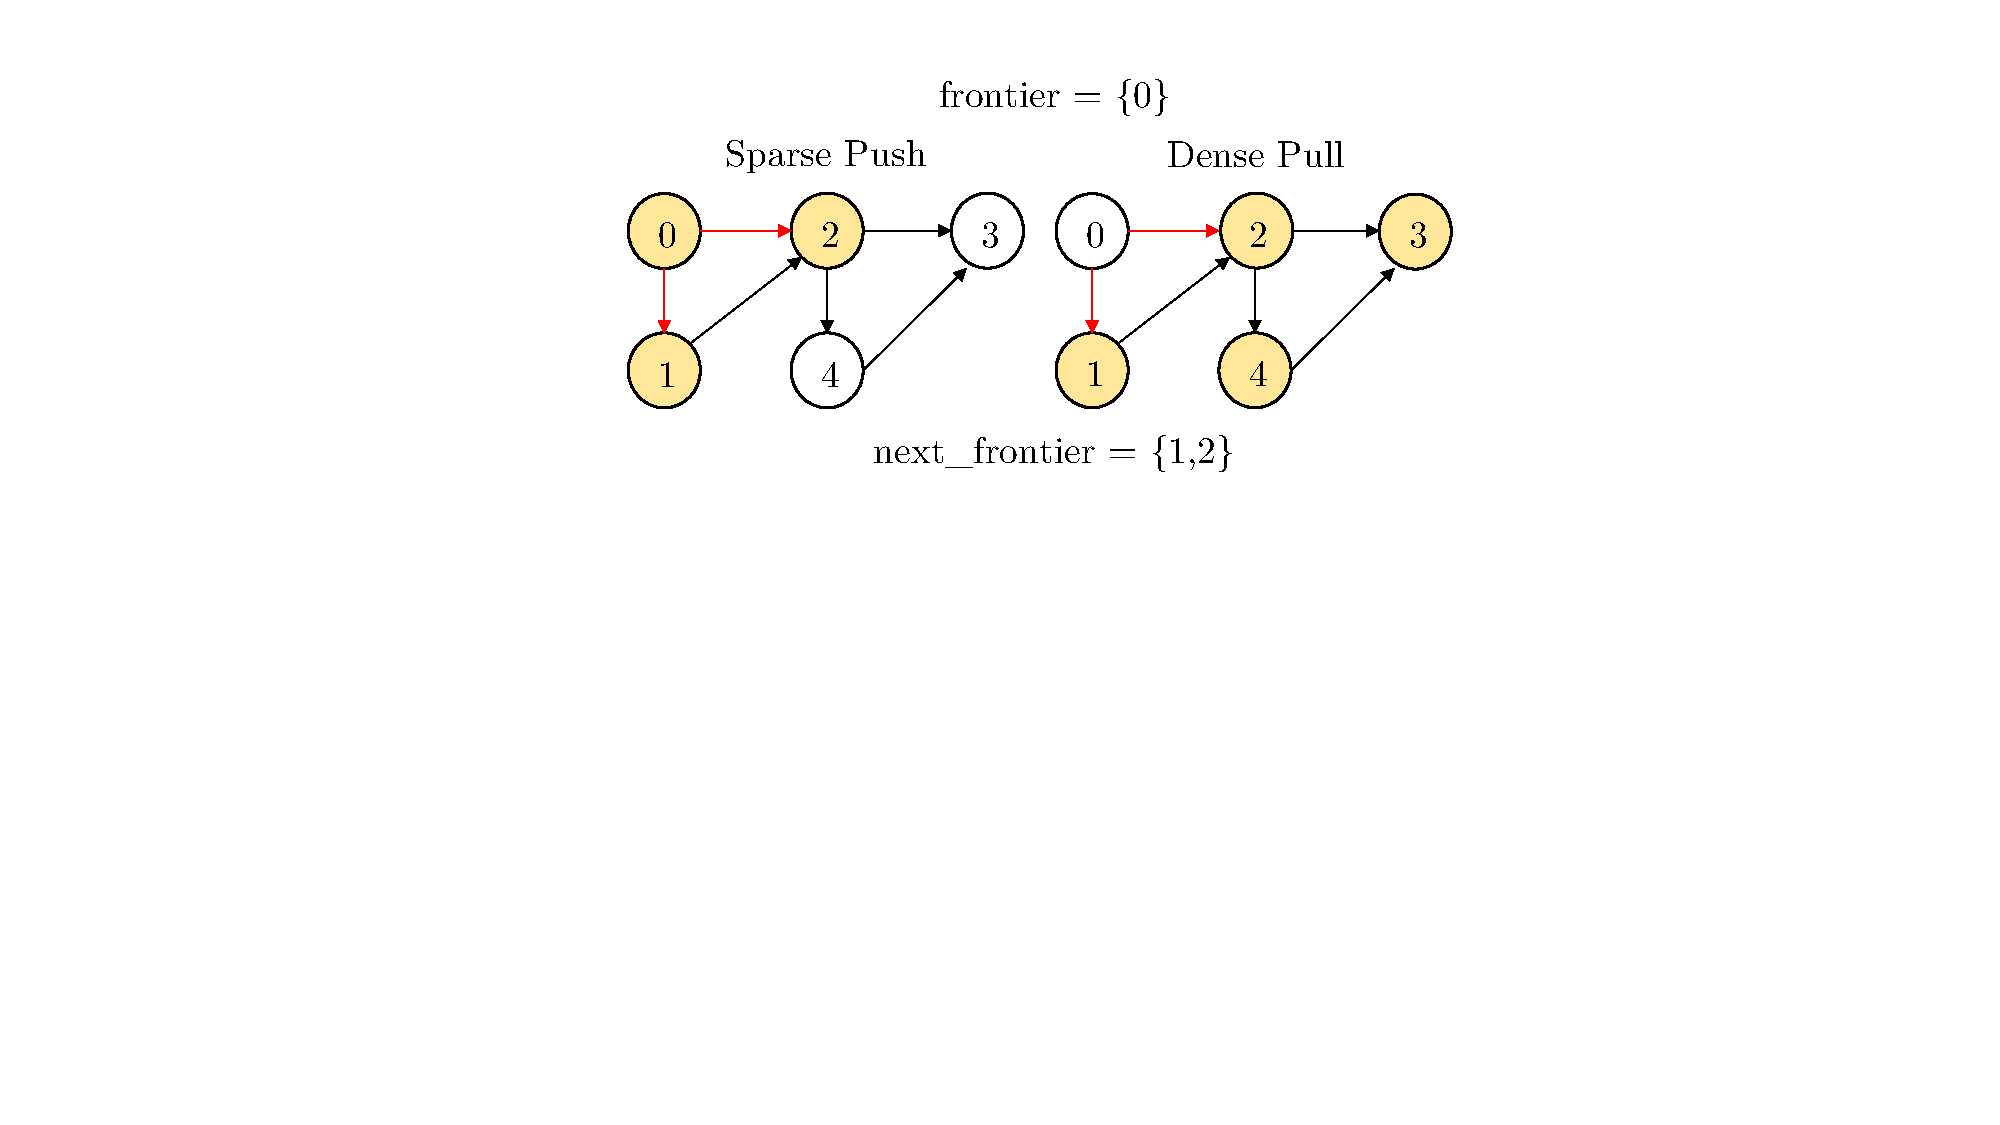
\includegraphics[scale=0.7]{graphit-figures/push_v_pull_fig.pdf}
    \caption{Representation of one iteration of BFS in both the \textsc{Push} and \textsc{Pull} directions. Nodes highlighted in yellow are visited during the iteration. Edges in red are edges that are traversed during execution.}
    \label{fig:pushpull}
\end{figure}
}

In this chapter, we explore optimizations to improve graph application performance on the manycore system described in Chapter~\ref{pap:generals:sec:architecture}.
First, we discuss a blocked access method for graph data to better exploit memory-level parallelism (MLP) in software.
Next, we present three different work partitioning schemes.
We then introduce a new frontier storage format that targets very sparse frontiers. 
%Next, we discuss an implementation of edge-aware vertex partitioning. 
We follow this with an exploration of graph traversal directions.
%Lastly, we introduce a GraphIt backend for a manycore architecture which can automate the process of applying the schedules discussed in this section. 

\section{Blocked Access Method}\label{sec:method:sub:blocked}
%\combinedBlockingFigure
%Figure \ref{pap:generals:sec:method:sub:blocked:fig:blocking}(a) shows the data layout of BFS on the manycore.
In the naive execution model, cores request single words of application data at the time of use.
The LLC responds to these requests, fetching data from HBM main memory when there is a cache miss.
We discover from profiling that applications spend most cycles waiting on serialized read requests from LLC and DRAM.
Many of these loads occur in iterations of the outer loop between which there are no data dependencies.
%This motivates an optimization in which software reschedules these long-latency memory requests to happen in parallel.
%\nonblockedMethodFigure

\blockedMethodFigure

Software can reschedule these long-latency requests to execute in parallel by formatting work items into blocks.
Cores iterate over their assigned blocks, prefetching the entire block at once.
The block data is stored in the core's scratchpad memory, re-purposing it as a software managed L1 cache.
Figure~\ref{pap:generals:sec:method:sub:blocked:fig:blocked} illustrates the blocked memory access technique. 
Work items are stored in HBM in contiguous cache-aligned blocks.
The LLC fetches a block from DRAM after receiving an initial load request from software.
Cores issue these memory requests with an explicit call to \lstinline[language=C++, basicstyle=\small\ttfamily]{memcpy} to exploit pipelined non-blocking loads and hide memory latency.
After fetching the blocked data, cores complete the loaded work before continuing to the next block.
Cores must flush modified blocks back to main memory before fetching the next block.

This blocked access method gives software fine grain control over what data is read at the block and word granularity allowing the application to only prefetch data it is likely to use. 
%For graph applications, this provides benefits when performing random read-modify-writes by increasing the effective memory bandwidth. 
This improves effective cache bandwidth by eliminating false sharing between work items and improves core memory access latency by improving locality for a work item.
%This allows graph applications to take advantage of the spatial locality in the CSR data structure while avoiding over-fetch from performing random updates. 
%For graph applications, this removes over-fetching from random read-modify-writes even as software benefits
%\blockedMethodFigure

% Non-stalling memory operations improves this microarchitecture.
% The \lstinline[language=C++, basicstyle=\small\ttfamily]{memcpy} invoked by software for performing blocked accesses is finely tuned to issue many of these non-stalling loads at once.
% This provides the software with an easy way to exploit the system's MLP.
% Overlapping the time waiting for memory requests to make their way through the network and memory system improve single core performance.

%This blocked memory access optimization has two benefits over a system with hardware managed L1 caches.
%First, it removes the need for hardware to maintain cache coherence, which is hard to scale to a large number of cores \cite{agarwal1988cachecoherence}.
%Second, it gives software finely grained control over what data is read at the block and word granularity.
%As a result, this means applications only need to pay for prefetching data that it is likely to use.
%For graph applications, this blocked memory access method provides benefits when performing random read-modify-writes, as prefetched data in this case is unlikely to be used.

\section{Work Partitioning} \label{sec:method:sub:edge-aware-partitioning}


We implement and explore the two load balancing methods: vertex-based and edge-aware vertex-based partitioning. We also propose our own manycore specific work partitioning method: alignment-based partitioning. 

\paragraph{Vertex-Based}\mbox{}\\
In vertex-based partitioning, all cores receive an equal number of vertices to traverse. 
In real world graphs, the number of edges per vertex can vary drastically, and due to this, the vertex-based approach can lead to workload imbalance. 

\paragraph{Alignment-Based} \mbox{}\\
In alignment-based partitioning, cores work instead on smaller work blocks of vertices that better align with cache lines in the LLC and make better use of the entire memory system by increasing effective bandwidth.
In this method, the vertices in the graph are split into $V/b$ work blocks where $b$ is the number of vertices contained in each work block and $V$ is the total number of vertices in the graph. We select $b$ to be a multiple of the cache line size. By doing this and by reducing the size of the active set of vertices that each core is working on, we are able to increase the cache hit rate and reduce cache line contention.

%This partitioning scheme reduces the size of the active set of vertices that each core is working on at any time.

\paragraph{Edge-Aware Vertex-Based}\mbox{}\\
\edgeAwareMethodFigure
Edge-aware vertex partitioning scheme considers the number of edges being assigned to each core when partitioning the vertices.
Figure~\ref{fig:edgeaware} demonstrates how edge-aware partitioning differs from vertex-based.

In Figure~\ref{fig:edgeaware}, Partition 1 shows a vertex-based partitioning and Partition 2 represents an edge-aware partitioning of the graph.
In both cases, the number of vertices assigned to each core is 5, but in the vertex-based partitioning scheme the first core is assigned 8 edges and the second core is assigned 21 edges.
This could lead to a large workload imbalance.
In the edge-aware partition, the first core is assigned 14 edges and the second core is assigned 15.
By considering the number of edges being assigned to each core, edge-aware partitioning is able to create a more balanced workload across cores.

\edgeAwareMethodAlgorithm

In order to accomplish edge-aware vertex-based partitioning, a maximum number of edges that can be assigned to a core is set before execution, we refer to this maximum value as the grain size.
Edge-aware partitioning effectively does a binary search for partitions of vertices that do not exceed this maximum number of edges. 
Initially, all vertices are considered in one large partition.
%In the first iteration, the core attempts to assign all of the vertices in the graph to itself. 
If this partition of vertices exceeds the number of edges that can be assigned to a core, it is split in half, and each of those partitions are examined as possible candidates.
This process continues recursively until all vertices have been assigned to a core.
The pseudocode for this recursive call is shown in Figure~\ref{alg:edge-aware}.

In our implementation, a single core is tasked with performing the recursive assignment of work while the remaining cores wait to receive their work assignment. 
Further, the grain size in our implementation is set to $(E / N) * 1.5$ where $E$ is the total number of edges in the graph and $N$ is the number of cores in the manycore. 
We found that a buffer value of $1.5$ was necessary to ensure that all of the vertices were assigned across the cores for all sizes of $E$ and $N$ that we examined.
While there is overhead introduced by this partitioning scheme, we expect that a more balanced split of work will improve load balance and memory system performance on graph programs with unbalanced input graphs.

%\edgeAwareMethodAlgorithm

%Figure \ref{alg:edge-aware} shows the pseudocode for this assignment routine.
%In the first iteration, the core attempts to assign all of the vertices in the graph to itself.
%If the number of edges is greater than the grain size, the recursive call is made.
%In the recursive call, the number of vertices in the range is split in half and the core checks if either the first half of the vertices or the second half of the vertices can be assigned to any core. 
%If either of them contain too many edges, the recursive call is made again.


\section{Bucketed Sparse Frontier}
A common optimization when traversing in the \push direction is to use a sparse frontier of length $m$ where $m$ is the number of active vertices and each element corresponds to an active vertex.
In contrast, a dense frontier is often used in the \pull direction where the frontier is stored as a boolean list of length $|V|$ and a value of \lstinline{true} indicates an active vertex.

In order to maintain some locality and to easily partition work across cores, our code generator defaults to a dense frontier in both directions.
However, this can lead to unnecessary cycles spent checking every vertex to see if it is in the frontier.
To address this, we propose a bucketed sparse frontier storage format. 
In this format, the frontier is still of length $|V$ and is split into $n$ buckets where $n$ is the total number of cores.
Each bucket stores a list of the active vertices in that range followed by $-1$s to indicate the end of active vertices in that bucket.
This allows us to use our vertex-based partitioning scheme while reducing the number of reads to the frontier.

\section{Graph Traversal Directions}

\pushVPullMethodFigure

In traditional Breadth-First Search, the graph is traversed in a top-down manner by examining the outgoing edges of vertices in the frontier.
For each vertex in the frontier, its edges are traversed and previously unvisited destination vertices are added to the next frontier.
As the size of the frontier grows, the number of edges that need to be traversed also increases.

Beamer et al.~\cite{beamer-bfs-direction} introduced a new method of traversal that reverses the direction in which edges are examined, and showed that this bottom up \pull approach can greatly reduce the number of edges traversed and improve performance. 
In this case, the edges of every vertex in the graph are examined, looking for vertices that are in the current frontier.
There are algorithmic optimizations that can be made in the \pull~direction to reduce the number of vertices and edges that are examined though. 
In BFS for instance, if a node has already been visited in a previous iteration, its edges do not need to be examined in any subsequent iteration.

Figure~\ref{fig:pushpull} shows both the \push~and \pull~directions for one iteration of BFS on a small graph.
In this example, we start the iteration with vertex 0 in the frontier. 
In the \push~case, the outgoing edges of vertex 0 are examined first.
Because vertices 1 and 2 have not been visited before, they are added to the next frontier.
In the \pull~case, all vertices that have not yet been visited are examined.
In this case, the incoming edges of all vertices except vertex 0 are traversed.
If an edge originates at a vertex that is in the current frontier, the destination vertex is added to the next frontier.
In Figure~\ref{fig:pushpull}, vertices 1 and 2 have edges that originate at vertex 0, so they are added to the next frontier. 

Beamer et al.~\cite{beamer-bfs-direction} find that while the \pull~direction increases performance on dense frontiers, traversing the graph in the traditional top down \push direction is still the better option on sparse frontiers and propose a \hybrid~traversal method.
The \hybrid~approach examines the size of the frontier for each iteration in order to determine whether to execute in the \push~or \pull~direction for that iteration.
Our code generator supports generating code in the \pull, \push, and \hybrid~directions.
%In the \push~direction, the graph is traversed first by the vertices in the current frontier.

The original hybrid traversal method proposed by Beamer et al. involves two different heuristic conditions~\cite{beamer-bfs-direction}. 
One for initially switching from \push to \pull and one to switch back to \push again towards the end of execution. 
These heuristics are based on: the number of vertices in the graph $n$, the number of edges in the graph $m$, the number of vertices in the frontier ($n_f$), the number of edges to check from the frontier ($m_f$), and the number of edges connected to unvisited vertices ($m_u$).
Each of these conditions also have parameters that can be tuned to best fit the target architecture. 
The first condition is defined as:
\[ m_f > \frac{m_u}{\alpha}\]
In their initial tuning study on a dual-socket Intel Ivy Bridge server, Beamer et al. select $\alpha = 15$ for optimal performance.
The second condition to switch back to the \push direction at the end of execution is:
\[ n_f < \frac{n}{\beta}\]
Here, the original tuning study found $\beta = 18$ to be optimal in most cases. 
With these $\alpha$ and $\beta$ values, Beamer et al. found that their hybrid heuristics provided an average speedup of $3.4\times$ over a \push implementation~\cite{beamer2016thesis}. 

The Ligra system~\cite{shun2013ligra} introduced a simplified heuristic to switch between the \push and \pull directions. 
Ligra also added functionality to switch between dense and sparse frontier representations given the traversal direction.
The condition for switching directions in Ligra is defined as:
\[ n_f + m_f > \frac{m}{\alpha}\]
Where again $n_f$ is the number of vertices in the frontier, $m_f$ is the number of edges to check from the frontier, and $m$ is the number of edges in the graph. 
In the Ligra implementation $\alpha = 20$. 
This heuristic doesn't require the application to maintain extra state to track whether the application has switched from \push to \pull, and removes the calculation of $m_u$.
With this much simpler code, Ligra is able to achieve close to the same performance as the hybrid traversal method introduced by Beamer et al~\cite{shun2013ligra}.

%\subsection{Traversal Parameter Tuning}

\section{Chapter Summary}

In this chapter, we described graph processing optimizations that seek to improve performance on the \hb~manycore through data layout, memory access patterns, and graph traversal direction.
First, we introduced the blocked access method for graph data that utilizes scratchpad memory and better exploits memory-level parallelism (MLP) in software.
Next, we discuss three different work partitioning schemes: vertex-based, edge-aware vertex-based, and alignment-based.
Vertex-based and edge-aware vertex-based are existing optimizations that we adapted for the \hb architecture, and alignment-based partitioning is a scheme that we developed to better exploit MLP.
We then introduced the bucketed sparse frontier that reorganizes frontier data to improve performance on very sparse frontiers.
Finally, we discussed graph traversal directions and two different hybrid traversal algorithms.
%Next, we discuss an implementation of edge-aware vertex partitioning. 
%We follow this with an exploration of graph traversal directions.